

\chapter{DOMINANCE EPISTASIS AND SELECTION}

In any concerted attempts to describe the effects of changes in genetic parameters on some systemic measure of the whole system, the phenomena of dominance and epistasis becomes a problem which demands `explanation'. Not only is it. a problem to the `Mendelian' geneticist insofar as he is concerned with the mechanism of gene action but it has been the concern of the `quantitative' geneticist insofar as he is concerned with tho selection and maximisation of some desirable character. It is immediately obvious that the treatment of biochemical systems, so far attempted, makes it in principle possible to reformulate the question in molecular terms. Given that we can formulate the dependance of some measure on the quantitatively specified parameters of a locus-specific enzyme, we. can investigate the changes in the measure when substitutions at this locus occur.

As before, it is worth mentioning how far the relatively abstract treatment may be relevant to the phenomena well known in `real' organisms. The characters of economic interest, such as growth rate, milk yield etc. cannot, of course, be specified precisely in biochemical terms. It is, however, generally agreed that the rate of synthesis of the various 'end products' is intimately related to the `flux' through this different pathways leading to them. In these studies this flux was therefore taken as the 'character' since the kinetic formulation in terms of the constituent enzyme activities (and hence the genes) can be given.

Similarly dominance can be measured by observing the effect on this flux of successive substitutions at the locus. Or again epistasis, regarded as the strength of interaction between different loci, can be estimated by observing how the response of the flux to substitution at one locus is influenced by a simultaneous substitution at another. One result which will be demonstrated is that a considerable. degree of dominance and interaction almost invariably arises even when the simplest assumptions are made about the properties of the individual enzymes. With more complex (and more realistic) assumptions, such as saturation, divided pathways and feedbacks, these interactions are even stronger. This appears to arise merely from the fact; true for all organisms, that enzymes are always embedded within a metabolic network of some sort. This seems particularly interesting in the case of dominance since it suggests that the common occurrence of dominance is not in need of a theoretical explanation, (such as the ``evolution of dominance''), arising as it does from the general nature of metabolism common to all organisms.

In addition an attempt will be made to understand the implications of this `gene-interaction' for the response to selection on the flux, for a `population' of such `organisms'.

Two aspects of such an investigation, however, require special treatment which, so far, it has not been necessary to consider in detail. The first is a method of handling a diploid situation, the second the fact that we shall, in general, be concerned not with differential changes but with discrete (and perhaps `large') steps in the parameter space.

As a first attempt to include diploidy and discrete parameter changes within a theoretical treatment it was realised that an analytic study of a straight chain of simple `linear' enzymes, when thps flux through the chain can be found algebraically, might be of considerable general interest. Such a system, whilst always an oversimplification, allows fully for genes, acting via enzymes which are embedded in a metabolic network, and therefore can be expected to possess the type of irreducible interaction which is common to all organisms. Consequently properties of such a system can be regarded as having a fairly general bearing whenever alleles at many loci contribute, within a given metabolic system, towards a character. Such a treatment will now be given.

\section{Dominance and epistasis in a straight chain of enzymes}

In order to discuss the response of the flux through the chain of enzymes to the various allelic substitutions it is necessary to define certain quantities. Firstly, there is the quantity of ``allelic swing'' or, $\lambda$, which measures the ratio between the high enzyme activity of the `good' allele and the low activity of the `bad' one at any particular locus. The allelic swing can, of course, have different values at different loci. Secondly, there is the quantity measuring the importance of a particular enzyme step in controlling the flux through the pathway namely the sensitivity coefficient.

Finally there is the ``maximum response to selection'', $R$, measuring the ratio between the flux of the `best' organism (all alleles good) and the worst (all alleles bad). 

Consider now the straight chain system indicated below:

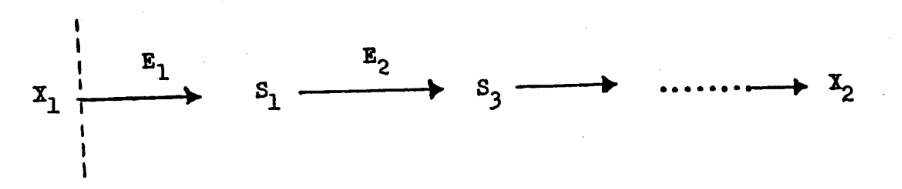
\includegraphics[max width=\textwidth, center]{figure5_1}

The diagram shows the conversion of a precursor at constant concentration $X_1$ into a product at constant concentration $X_2$ via a sequence of enzymatically catalysed steps $\mathrm{E}_1, \mathrm{E}_2 \ldots$ etc. The concentrations of the metabolic intermediates being $S_1, S_2$, . etc. At the stationary state, when the intermediates have all stopped changing, the pathway will produce $X_2$ from $X_1$ at a steady rate, $F$, where $F$ is the net-flux in the pathway.

In addition we must specify the enzyme activities corresponding to the two alleles, namely $V^H$ and $V^L$. Furthermore the allelic state at any one locus is specified by a number.

\begin{center}
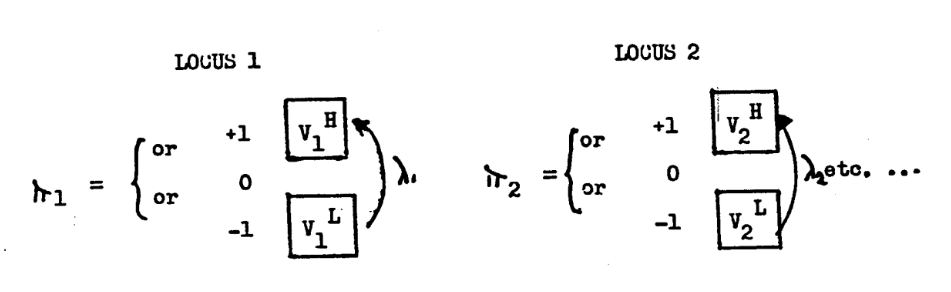
\includegraphics[max width=\textwidth]{figure5_locus.png}
\end{center}

The set of numbers $\pi_{1}, \pi_2,$ etc. can each take one of three values. Thus, $\pi=-1$ corresponds to the homozygote having the low activity enzyme, $\pi=0$ to the heterozygote and $\pi=1$ to the high activity homozygote. The set of integers $\pi_{2}, \pi_{2}$, etc. thus specify the genotype of the `organism', and a finite population of organisms is specified when the $\pi$ vector of each organism in the population is known.

The enzymes are assumed to convert substrate into product at a rate given by a \underline{linear} expression of the form $f = V(A-B/K)$, where $V$ is the activity of the enzyme, $K$, an equilibrium constant, and $A$ and B the concentrations of its substrate and product. This corresponds to an unsaturated `Michaelis' type enzyme, and, on the assumption that enzyme concentration is proportional to gene: dosage, the heterozygous state at the ith locus will \underline{also} be represented by a linear rate expression having an `activity' $V_{i}^{*}$, midway between the low and high activities $V_{i}{ }^{L}$ and $V_{i}^{H}$. It can be shown, CH.I, that if the effective activities, $V_{i}$, at the separate steps are measured in appropriate units the flux $F$ through the pathway is given by
%
\begin{equation}
F = \left(X_{1}-X_{2}\right) / \sum \frac{1}{V_i}
\label{eqn:501}
\end{equation}
%
The effective activity at the ith locus can now be written in terms of $V_{i}^{*}$, its heterozygous value, $\pi_i$ and which indicates the allelic state at the locus and $\lambda_{i}$ the allelic swing at the locus. Thus since $\lambda_{i}$ is the ratio between the high and low activities at the ith locus we have
%
$$
\lambda_{i}=\frac{V_{i}^{H}}{V_{i}^{L}} \text { and }{V_{i}^{*}} = \frac{{V_{i}^{H}} + V_{i}^{L}}{2}
$$
%
From this it follows that
%
$$ V_i^H = V_i^*\left(1+\frac{\lambda_i-1}{\lambda_i+1}\right) $$
%
and 
%
$$V_{1}^{L}=v_{1}^{*}\left(1 - \frac{\lambda_{i} - 1}{\lambda_{i}+1}\right)$$

The activity corresponding to the ith locus, $V_{i}$, can now be written, using $\pi_{i}$ the genotype variable for the ith locus, as:
%
\begin{equation}
V_{i} = V_{i}^{*}\left(1+\pi_{i} \frac{\lambda_{i}-1}{\lambda_{i}+1}\right)
\label{eqn:502}
\end{equation}
%
where $\pi=-1$ means the low homozygote, $\pi=0$ means the heterozygote and $\pi+1$ means the high homozygote.

Combining this with (5.1) and introducing $\beta_{i}=\frac{\lambda_{i}-1}{\lambda_{i}+1}$ we get 
%
\begin{equation}
F=\left(X_{1}-X_{2}\right) / \sum \frac{1}{V_{i}^{*}\left(1+\pi_{i} \beta_{i}\right)}
\label{eqn:503}
\end{equation}
%
When the genotype is known, that is the values of $\pi_i$ are specified for each locus, the flux through the system can be found using relation (5.3). Thus for the rather simple system under consideration we have now an explicit formula relating the measure $F$ and the logical vector $\left(\pi_{1}, \pi_{2}\right.$,...) which specifies the genotype. This genotype/phenotyp mapping function, based on biochemical considerations, can now be used to consider what sort of gene interactions are likely to be significant in this system.

\section{Dominance}

The response of the flux, measured in suitably scaled units, to successive alterations, made at locus I for example, can be used to consider dominance in the model. Thus by using the expression (5.3) and collecting together all terms not directly affected by the 1st locus we have -
%
$$\mbox{writing } a_{1}=\sum_{i \neq 1} \frac{1}{V_{i}^{*}\left(1+\pi_{1} \beta_{i}\right)} $$
%
$$ a_{2}=X_{1}-X_{2} $$
%
\begin{equation}
F = a_{2} / a_{1}+\frac{1}{V_{1}\left(1+\pi_{1} \beta_{1}\right)}
\label{eqn:504}
\end{equation}
%
The rate controlling effect of the 1st enzyme can be found as -
%
\begin{equation}
C_{V_{1}}^{F}=\frac{V_{1}}{F} \cdot \frac{d F}{d V_{1}} = \frac{1}{V_{1}\left(1+\pi_{1} \beta_{1}\right)} /\left(a_{1}+\frac{1}{V_{1}\left(1+\pi_{1} \beta_{1}\right)}\right)
\label{eqn:505}
\end{equation}
%
Clearly since $a_{1}$ is a function of $\pi_{2}, \pi_{3}$, etc. the control effect of $V_{1}$, i.e the value of $C^F_{V_1}$, depends no the genetic background.

When the 1st locus is heterozygous (5.5) takes a particularly simple form. Thus for $\pi_{1}=0$ (i.e. heterozygous) at the let locus we have
%
\begin{equation}
\left(C_{V_{1}}^{F}\right)_{\pi_{1}=0}=\frac{1}{V_{1}} \big/\left(a_{1}+\frac{1}{V_{1}}\right)
\label{eqn:506}
\end{equation}
%
In order to consider the degree of dominance present at a locus a suitable measure of dominance is required, as for example that given by Falconer (1959); Thus if $\mathrm{F}_{-1}, \mathrm{F}_{0}, \mathrm{F}_{1}$ represent the flux corresponding to the low homozygote, the heterozygote and the high homozygote at the 1st locus, all on a given background, then the dominance is given as
%
\begin{equation}
\text { DOMINANCE }=D=\frac{F_{0}-1 / 2\left(F_{-1}+F_{1}\right)}{1 / 2\left(F_{-1}+F_{1}\right)-F_{-1}}
\label{eqn:507}
\end{equation}
%
Using this measure of dominance, complete dominance of the high activity allele would correspond to $D=+1$ and over-dominance to $D>1$, while $D=0$ indicates a purely additive response to successive substitutions at the 1st locus. The equation (5.4) giving the flux as a function. of the state of the Ist locus can now be used in conjunction with (5.7) to obtain an expression for the degree of dominance at the 1st locus.

This manipulation is made easier if (5.4) is rewritten a follows:
%
$$
\begin{aligned}
F & =a_{2} / a_{1}+\frac{1}{V_{1}\left(1+\pi_{1} \beta_{1}\right)} \\
& =a_{2}-\frac{a_{2}}{a_{1} \beta_{1} V_{1}} \cdot \frac{1}{\pi_{1}+1 / \beta_{1}\left(1+1 / a_{1} V_{1}\right)}
\end{aligned}
$$
%
\begin{equation}
F = a_{2}-K\left(\frac{1}{\pi_{1}+\gamma}\right)
\label{eqn:508}
\end{equation}
%
where 
%
$$K=\frac{a_{2}}{a_{1} \beta_{1} v_{1}} \quad \mbox{ and } \quad \gamma=\frac{1+a_{1} V_{1}}{\beta_{1}}$$
%
When substituting the appropriate expressions for $F_{-1}, F_{0}, F_{1}$ in (5.7) (i.e. giving values $-1,0+1$ for $\pi_{1}$ in $(5.8)$ ) the leading term of unity and the factor $K$ cancel out and we get:
%
$$
D = \frac{F_{0}-1/2\left(F_{-1}+F_{1}\right)}{1/2\left(F_{-1}+F_{1}\right)-F_{-1}} = \frac{1}{\gamma}-\frac{1}{2} \left(\frac{1}{1+\gamma} + \frac{1}{-1+\gamma}\right) \bigg/ \frac{1}{2}\left(\frac{1}{1+\gamma} + \frac{1}{-1+\gamma}\right)-\frac{1}{-1+\gamma}
$$
%
which on simplification yields $\quad D=\frac{1}{\gamma}$

remembering that
%
$$
\beta_{1}=\frac{\lambda_{1}-1}{\lambda_{1}+1} 
$$
this becomes
$$
D=\frac{\lambda_{1}-1}{\lambda_{1}+1}\left(\frac{1}{1+1 / a_{1} V_{1}}\right)
$$
%
which can be further simplified by using (5.6) to replace the factor
%
$$ \frac{1}{1+1 / a_{1} V_{1}} \mbox{ resulting in } $$
%
\begin{equation}
D = \frac{\lambda_{1}-1}{\lambda_{1}+1}\left(1-\mathrm{^{*}C}_{\mathrm{V}_{1}}^{\mathrm{F}}\right) \\
\label{eqn:508}
\end{equation}
or, in general 
$$
\mathrm{D}=\frac{\lambda_{-1}}{\lambda_{+1}}(1-\mathrm{C})
$$
The dominance of the locus thus is seen to depend both on its "allelic swing", $\lambda$, and on its heterozygous coefficient `C' (i.e. its rate controlling influence).

In this formula $C$ stand for the rate controlling influences of the 1st enzyme at its heterozygous position. The influence of the \underline{other} loci on the dominance of the first locus thus depends on their
influence on the rate controlling effect, $C$; of the first locus (ce. equation 5.6).

The formula (5,10) is quite general and indicates that the dominance measure at a locus having a small rate controlling effect is almost independent of the background genotype, the small value of $C$ having only a small effect on the factor $(1 - C)$, and depends directly on the $\lambda$ for the two alleles at the locus in question. Let us consider the `symmetrical case' where many loci have similar enzyme activities and $\lambda$ values. In this case the `maximum response to selection', R, will define the $\lambda$ values. By `response' is meant the ratio between the flux of the best organism (all alleles `good') and the worst organism (all alleles `bad'), and inspection of relation (3) for the two cases indicates that the separate $\lambda$ must all be approximately equal to $R$.

For the many locus symmetrical case we have, therefore; for each locus
%
$$D \bumpeq \frac{R-1}{R+1} \mbox{ and } C \mbox{very small.} $$

Thus for a population of organisms where the $n_{\text {maximum response }}$ $R$, is reasonably large, the dominance can be almost \underline{complete}, even though the effects of inhibition at the individual loci have become vanishingly small.

\section{Epistasis}

A similar approach can be used to consider the importance of interlocus interactions or epistasis within the same model system. In this case a suitable measure of the interaction between two loci is the increment in flux when both act together over that which would be expected from the sum of their separate effects.

If $F_{00}$ represents the flux with both loci homozygous low, $F_{01}$ with one homozygous high and similarly for $F_{10}$ and $F_{11}$ then the epistatic interaction `$E$ ' may be defined as -
%
\begin{equation}
\mbox{EPISTASIS } = \mathrm{E} \frac{\left(F_{11}-F_{00}\right)-\left(F_{10}-F_{00}\right)-\left(F_{01}-F_{00}\right)}{\left(F_{10}-F_{00}\right)+\left(F_{01}+F_{00}\right)}
\label{eqn:510}
\end{equation}
%
In terms of the measured increment, $F_{M}$, and the increment, ${F}_{AD}$ which would be expected if the loci acted additively this can be written as
%
$$
E=\left(F_{M}-F_{A D}\right) / F_{A D}, \quad \text {so that:} \quad F_{M}=F_{A D}(1+E) \text {. }
$$
%
The measure $\mathrm{E}$ will be zero if the loci act additively whereas 1f, for example, $E=1$ it means that joint action of the loci results in a $100 \%$ greater effect on $F$ than would be supposed on the basis of their additively.

It should now be possible, using (5.3), to substitute the various fluxes in $(5.10)$ and obtain an expression measuring interlocus interaction, just as was done for dominance interaction. However, this proves to be rather complex because we now have to consider coefficients and $\lambda$ ratios for each of two loci and the algebria is correspondingly. difficult. It is, therefore, advantageous to consider the case where the two loci have equal control effects and equal $\lambda$ ratios and interaction might be expected to be greatest. For this situation it is possible to show that -
%
\begin{equation}
E = C (\lambda-1) /(\lambda-2 C(\lambda-1)) \quad \ldots(5.11)
\label{eqn:511}
\end{equation}
%
where $C$ is the sensitivity coefficient of the flux with respect to either enzyme for the homozygous low or $F_{00}$ case and $\lambda$ is the allelic swing common to the two loci.

This formula shows that when there are many loci with about equal importance the interaction between pairs of loci will tend to zero. This is because $C$, the rate controlling effect of an individual Locus, becomes small as the number of loci increases. For the case of large $\lambda$ and $C \ll 1$ equation (5.11) becomes:
%
$$
\mathrm{E} \bumpeq \mathrm{C}
$$
%
Consider for example a symmetrical system with 10 enzymes acting in a chain, having a common $\lambda$ value greater than, say, 5. In such a system the coefficient $C$ of any locus will always be of order $0.1$ as also will be the epistatic interaction between any pair of loci. This means that simultaneous substitutions at any two loci will usually produce about $10 \%$ greater effect than would be expected from the sum of their separate effects. When there are a larger number of loci of about equal importance interactions between pairs of loci will tend to become negligible. However, this may hot be the case for interactions between more than two loci. A quick way of judging the importance of these high order interactions is to consider a mode? where the loci are split into two equal groups, each having a similar rate controlling effect and a similar $\lambda$. In this case the model formally reduces to a two enzyme pathway and the value of $C$ in (5.11) becomes $0.5$, since the rate control is shared equally between the two formal enzymes:
%
$$
\begin{aligned}
\mbox{thus} \quad \mathrm{E} &= \frac{0.5(\lambda-1)}{\lambda-2 \times 0.5(\lambda-1)} \\[5pt]
\mbox{or} \quad \mathrm{E} &= \frac{\lambda-1}{2}
\end{aligned}
$$

If $\lambda=10$ we have $\mathrm{E} \bumpeq 5$ which is a very marked gene interaction effect between, say, the first 10 and the last 10 loci in a pathway. 

We thus have a situation where high order interactions are quite marked at the, level of physiology of individual `model' organisms and this raises the question of the role of these interactions in the context of `population' genetics. Such questions can be considered most easily for the simple case of a symmetric model, that is for one in which substitutions made at one locus are exactly
equivalent to substitutions made at any other.

\section{Implications of study for response to selection}

Here, for simplicity, the physiologically symmetrical case will be considered, that is, all variable loci are assumed to have the same $V^{*}$ and $\lambda$ - Suppose that in the population there are $N$ such variable loci and in addition $V_{0}$ non variable loci each of which provides an effective activity having the same value as $\mathrm{V}^{*}$. In a particular organism let I loci have at \underline{least} on substitution by a `good' allele and of these let $I$ be the number of heterozygotes. The number of loci homozygous for the 'bad' allele will then be $(N-X)$ and the flux $F$ in such an organism will, using equation (5.3), be given by
%
\begin{equation}
F_{i}=\left(X_{1}-X_{2}\right) / \frac{No}{V^{*}}+\frac{N-X}{V^{*}_2/(1+\lambda)} + \frac{Y_{*}}{V^{*}}+\frac{\frac{X}{V^{*}}-Y}{V^{_{2}*} /(1+\lambda)}
\label{eqn:512}
\end{equation}

The value of $\mathrm{F}$ in different organisms will depend only on fixed parameters, having the same value for all the organisms, and on the proportion of loci in any particular organism which are singly or doubly substituted by the 'good' allele. Writing $x=\frac{X}{N}, y=\frac{Y}{N}, n=\frac{N o}{N}$ and dropping proportional factor: the relation $(5.12)$ can be written as
%
\begin{equation}
F \propto 1 \bigg/ 1+\left(\frac{2 n}{1+\lambda}\right)-x\left(\frac{\lambda-1}{\lambda}\right)+\frac{y}{\lambda}-\frac{2 \pi}{\lambda(\lambda+1)}
\label{eqn:513}
\end{equation}
%
When $\lambda$ is reasonably large (about 10) the relationship (5.13) will be well approximated by
%
\begin{equation}
F \propto 1 /(1+K-x)
\label{eqn:514}
\end{equation}
%
where
%
$$ K=\frac{2 n}{1+\lambda} $$
%
This approximate representation (5.24) describes a genotype-phenotype relation which is clearly \underline{dominant} at all loci, since $x$ is indifferent to a second substitution of a `good' allele. The importance of epistatic interaction in (5.14) can be seen by considering how the. response to a substitution depends on the background. Such a substitution represents a small increase, $\Delta x$, in $x$ and the response will be approximately given by
%
$$
\Delta F \approx\left(\frac{dF}{dx} \cdot \Delta x\right)
$$
%

$\displaystyle \mbox{or from (5.14)} \quad F \bumpeq \frac{1}{(1+k-x)^2} \Delta x$

thus for a given $\Delta x$ and using (5.14) again we have
%
\begin{equation}
\Delta F \propto F^2
\label{eqn:515}
\end{equation}
%
This means that for a population of such organism with a maximum response to selection $R$ of, say, 5 fold the effect of a given substitution can vary 25 fold ( $=5^2$ ) depending on the genetic background. The multiplicative interaction, often used to represent epistatic interaction in theoretical genetics, would give a response to substitution, analogous to $(5.15)$ of
%
\begin{equation}
\Delta F \propto F
\label{eqn:516}
\end{equation}

Clearly the relation (5.14) implies a `stronger' epistatic interaction than does a multiplicative model.

What does this imply for the behaviour of a finite population under selection for F? If the separate loci are very tightly linked on a single chromosome and the phenotype is defined in the dominant epistatic manner of (5.14) then selection will progressively reduce the number of chromosomes until only two or three chromosomal types remain. This is because with \underline{very} light linkage the system is equivalent to a large number of alleles at one locus and there are 'overdominance' relations between some of them. Selection thus leads to a reasonably complementary pair of chromosomes selected from among those originally present.

An argument will now be given to show that if such a pair of chromosomes predominate in the population a \underline{relatively} stable situation.

\begin{figure}
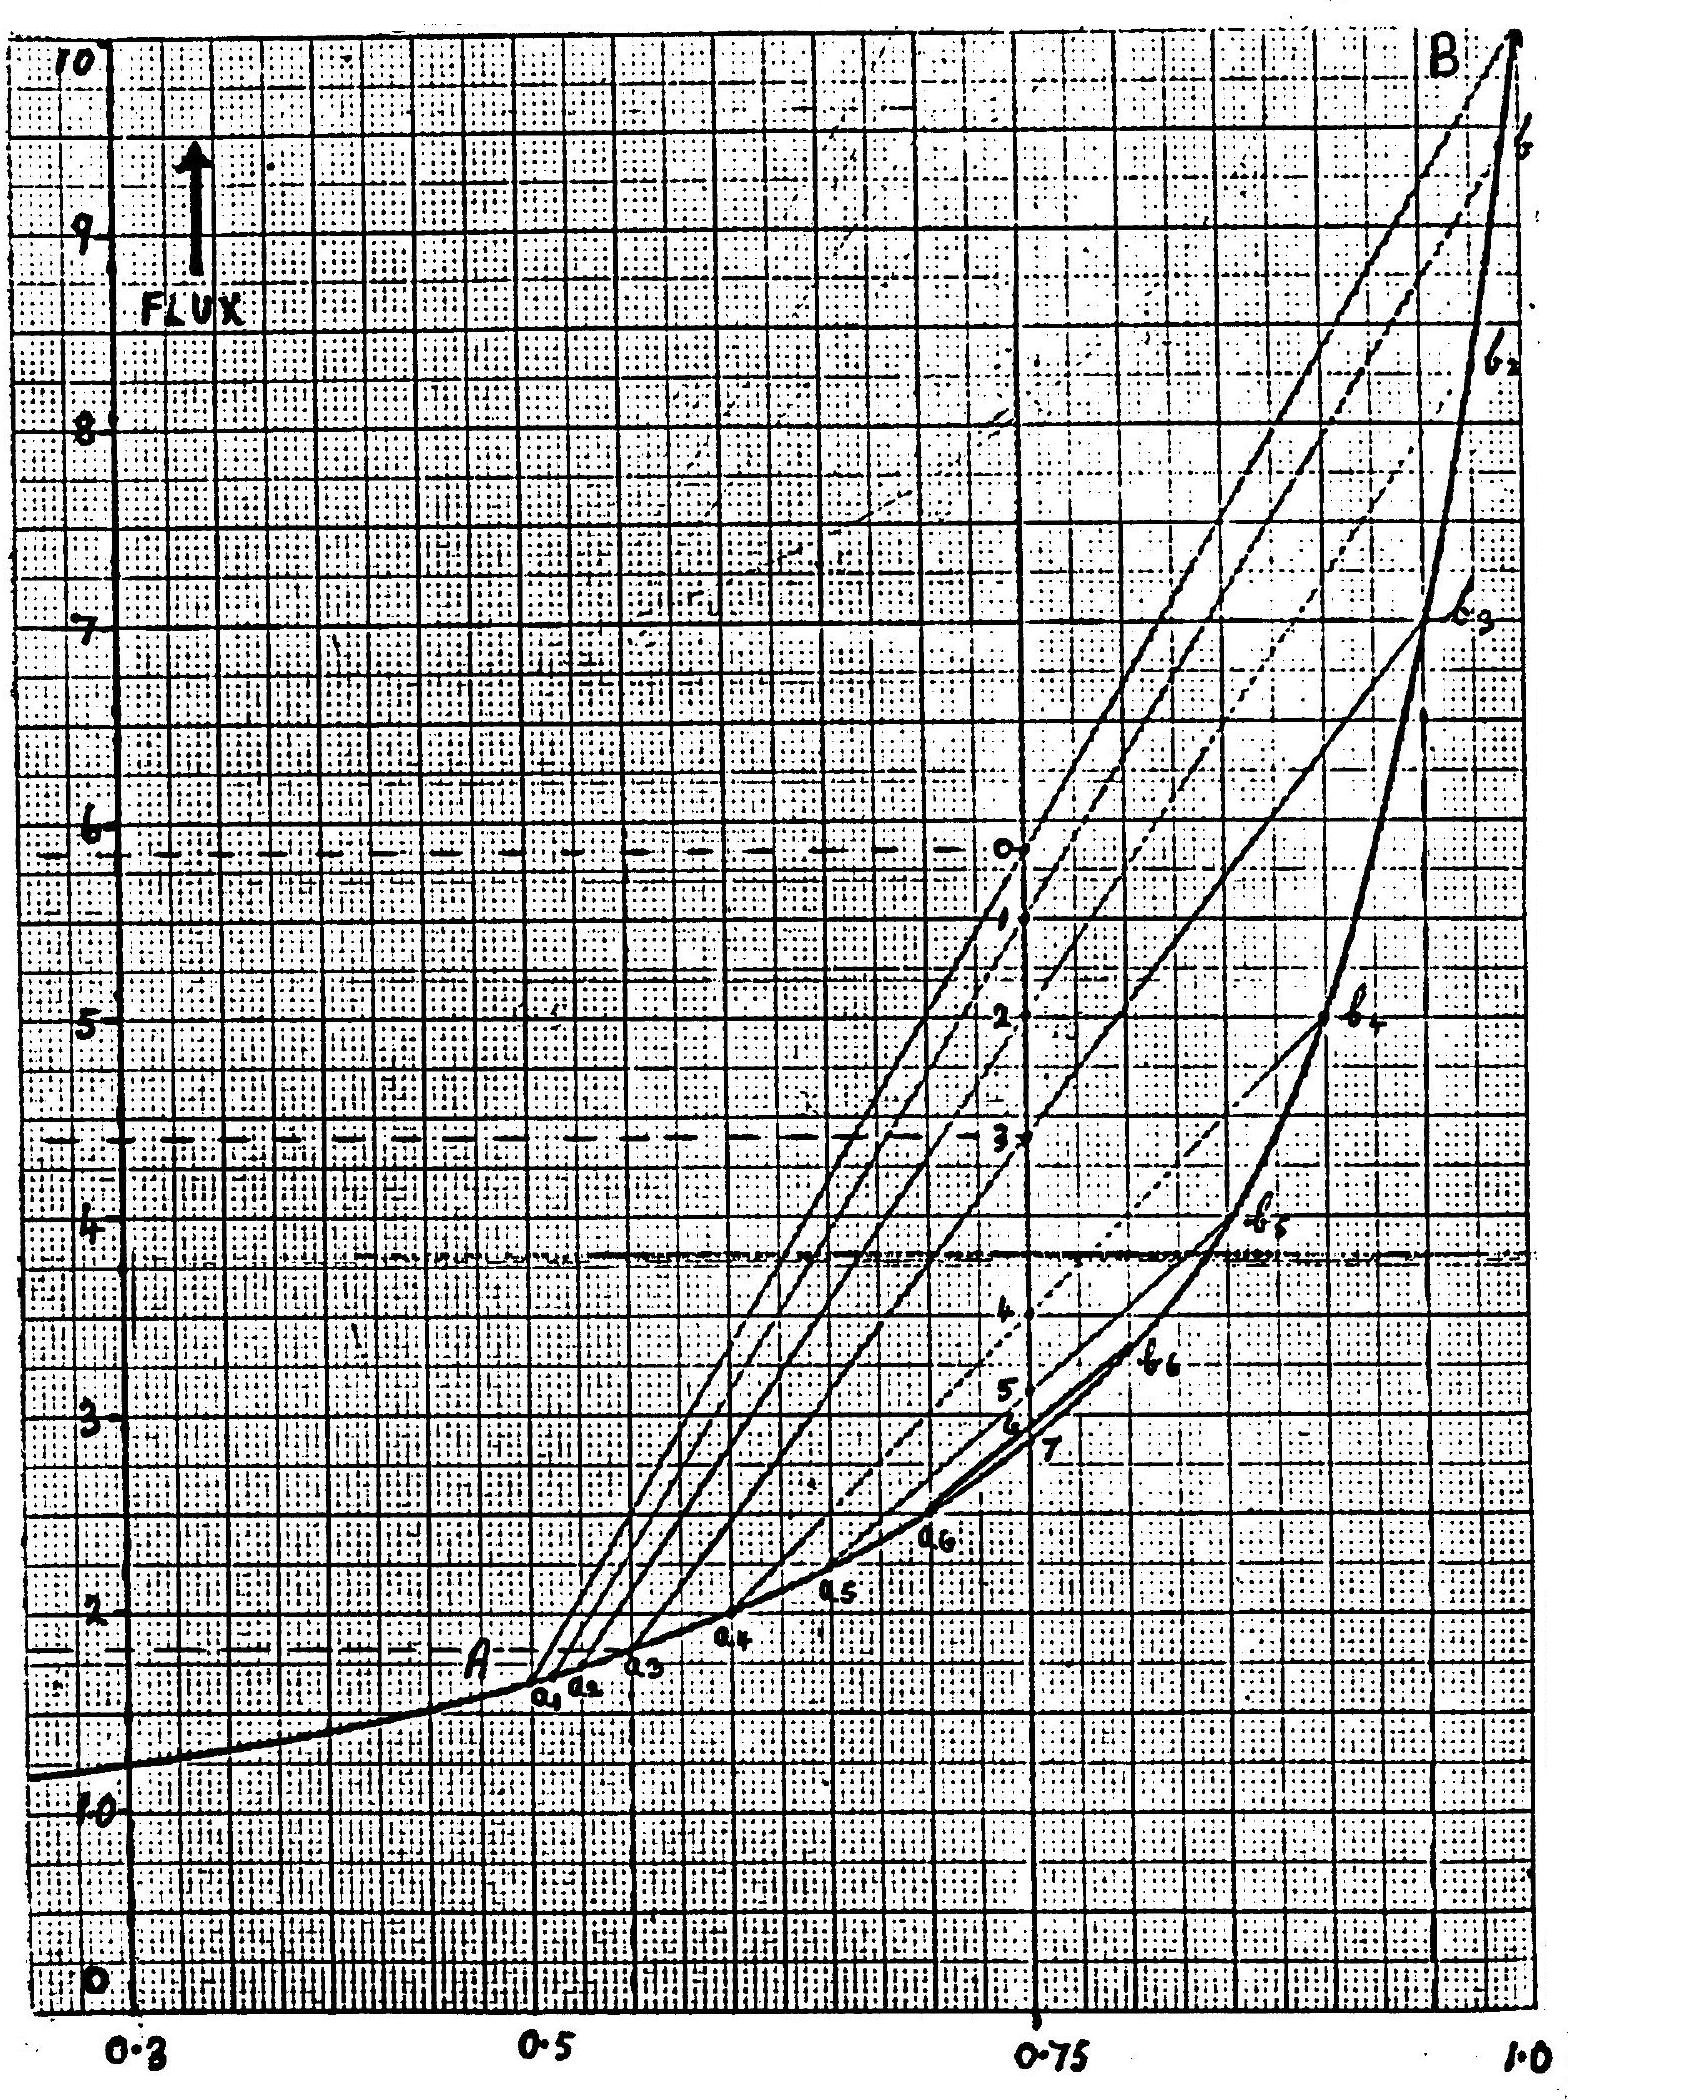
\includegraphics[max width=0.95\textwidth]{2023_01_30_a974a42f7b7381f3f940g-217}
\caption{The graph shows the plot of function (5.17). As an example consider a recombinant chromosome, formed by a cross-over occurring 1/10 from the end. This corresponds to the points a3 and b3 on the graph giving the point ``3''. This represents a mean value of 4.3 on the flux scale for this chromosome in the population compared to a value of 5.8 for either of the original chromosomes.
}
\end{figure}

may still exist even when recombination between chromosomes is allowed. Consider for example the relationship (5.14) when $n=1 / 2$, that is the ratio of non-variable to variable loci is $0.5$, and $\lambda=9$. Then
%
\begin{equation}
\text { F } \propto 1 /\left(1+\frac{1}{10}-x\right)
\label{eqn:517}
\end{equation}
%
This relationship between the flux and the proportion of substitutions, $x$, in a given organism is shown on the graph opposite, where $x$ moves almost continuously in the range zero up to unity when there are a large number of loci. Consider the limiting case when the number of loci is. large and the chromosome can be regarded as a continuous structure and, suppose, to keep the argument simple, that the two chromosomes have equal probability of good or bad alleles along their length and are complementary in the sense that a good allele in one always occurs opposite a bad allele in the other.

The argument regarding the `stability' of such a situation under upward selection for $F$ consists in showing that there will be strong selection against recombinant chromosomes and that these could therefore be removed as fast as they are produced. Thus consider the two predominant complementary chromosomes in the diagram below, which will be called `a' and `na', `na' standing for `not' a and suppose that a recombination occurs at a proportional distance `L' from one end. The new chromosome then consists of a portion, $L$, of `a' and a portion
$(1-L)$ of `na' as shown in the diagram below:

\begin{center}
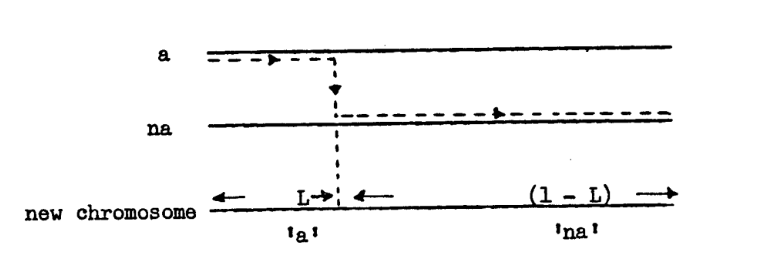
\includegraphics[max width=\textwidth]{figure5_chrom.png}
\end{center}

This new chromosome will occur in the population equally frequently with `a' and with `na' and hardly at all with itself. When combined with `a' its $x$ value will be $\left(1-\frac{L}{2}\right)$ and when paired with `na' its $\mathrm{x}$ value will be $\left(\frac{1}{2}+\frac{L}{2}\right)$, these points being symmetrically situated about the value $x=0.75$. The mean value of the new chromosome in the population will thus be found as the average or mid-point of the corresponding points on the graph, shown as $\left(a_{1}, b_{1}\right)\left(a_{2}, b_{2}\right)$, etc. for values of $L_{1}, L_{2}$ etc. which represent crossover positions increasingly close to the middle of the chromosome. The two predominant chromosomes `a' and `na' have identical mean values in the population. This value is equal to the mid-point of the line joining $A$ and $B$ on the graph, that is the point marked `0'.

Thus it can be seen that recombinant chromosomes corresponding to crossover near the middle of the existing chromosomes are at a strong selective disadvantage: Although the effect is less marked for crossovers near the ends of existing chromosomes the new chromosomes so produced will still be selected against. 

The general argument just given suggests that the combination of dominance and strong epistatic interaction, represented by the concavity of the graph of $F$ against $x$, can, when combined with reasonably close linkage, maintain a situation which is very far from linkage equilibrium. However, one important point has not been allowed for and this is that although it is reasonable to consider the chromosomes as continuous and balanced when considering crossovers within them this will not be so for crossovers at the extreme end.

In this case the new chromosome can actually become `better' than either of the existing ones, by picking up extra `good' alleles at its ends, and be selected in. This `end effect' should then lead to the gradual fixation of `good' loci, although this may happen very slowly since at any time only the outermost unfixed loci in the map are `available' for fixation.

It is, of course, important to see whether these qualitative predictions can be confirmed by direct simulation. A program capable of dealing with a reasonably large number of loci, say thirty, will be required if the `end effect' is to be observed and this has already been developed.

\section{The phenotype/genotype relation for more complex systems}

In CH II (p53-55) it was shown the genotype parameters, $\pi_1, \pi_2, \ldots$, could be embedded within the usual mathematical formulation of a complex metabolic system. The dependance of a phenotypic measure, $M_X$, on the genotype and the environment then being of the form
%
\begin{equation}
M_x = M_x\left(\pi_1, \pi_2, \ldots, \ldots, \pi_m, X_1, X_2, \ldots\right) \quad \ldots
\label{eqn:518}
\end{equation}

For the straight chain system just considered this took on the simple form of relation (5.3). In general, however, the relation cannot be expressed by a simple formula and it becomes necessary to employ the computer techniques of CH IV, both to construct and then investigate any particular system. In this way it is hoped that insight may be obtained into the way in which the underlying metabolic system determines general features of the $\mathrm{Ph} / \mathrm{Ge}$ relation.

Consideration of the analytically obtained expression (5.3) shows clearly that the general relation, (5.18), is unlikely to be approximated by any of the statistical representations commonly used in considering the behaviour of populations subject to selection for the quantitative character, as for example in Fraser (1962, 1967). How important this non applicability of the normally assumed $\mathrm{Ph} / \mathrm{Ge}$ relationship may be for population studies can be considered by running the usual simulation programmes of theoretical population genetics (Fraser, 1962) in conjunction with metabolic simulation programmes such as my own. However computational limitations soon arise. Thus a Monte-Carlo simulation of a 10 locus problem with an offspring population of 20 animals would take about 3 minutes/ generation compared with about 1/ 10 of a second for a symmetric non epistatic model on the same computer. This situation can be avoided by providing the population programme with a pre-computed table of phenotype values but this method becomes impractical at about 6 loci, (Burns, 1970). In these circumstances it remains important to consider the $\mathrm{Ph} / \mathrm{Ce}$ relationship at the physiological level in the hope of finding some relatively simple rules for compounding genetic effects operating through a metabolic network. However, even for such physiological studies. of models having alternative alleles at a number of loci, it is not always practical or useful to simply evaluate all the different phenotypes since there will be a very large number of these. In these circumstances the sensitivity coefficient can again provide useful insight, even though the $\pi$ variations are in fact finite. For example an estimate of the effect of a substitution at the ith locus, SUB $_1$, on a given background can be obtained as follows. Thus
%
$$
\mathrm{SUB}_i=\frac{\Delta M}{M} \bumpeq \frac{\partial M}{\partial \pi_i} \cdot \Delta \pi_i
$$
%
Since $\Delta t_{i}$ will be the same no matter what locus is being considered the relative importance of the different variable loci can be seen as
%
$$
\left[\mathrm{SUB}_{1}, \mathrm{SUB}_{2}, \ldots .\right] \propto \left[\frac{\partial M}{\partial \pi_{1}}, \frac{\partial_{1}}{\pi_{2}}, \ldots \ldots\right]
$$
%
The computer can easily produce the vector $\left[\frac{\partial M}{\partial{\pi_i}}\right]$ on various backgrounds and environments and hence reveal which genes have a major and which a minor effect and to what extent this classification is likely to be altered by changes in environment. In this respect the figure opposite, from a computer simulation of five saturable enzymes in a straight chain, shows how quite small changes in the environment can completely reverse the relative classification of two genes as major and minor.

\section{Dominance, when the allelic substitution has only a small effect on pools.}

In general two alleles at a locus will produce enzymes which are considerably different and complete substitution of one allele for the other can be expected to produce a marked change in at least some pools, although the effect on flux may be much less. Under these circumstances it is difficult to make any general argument about the degree of dominance, that is the position of the stationary solution corresponding to the heterozygous state at the locus.

Consider, however, the restricted case in which the alternative enzymes, whilst having distinct kinetic parameters, are each capable, at the existing steady state, of carrying about the same flux. It then becomes possible to relate the dominance to the two sensitivity coefficients corresponding to the locus being in the alternative homozygous states. The argument is as follows.

\begin{center}
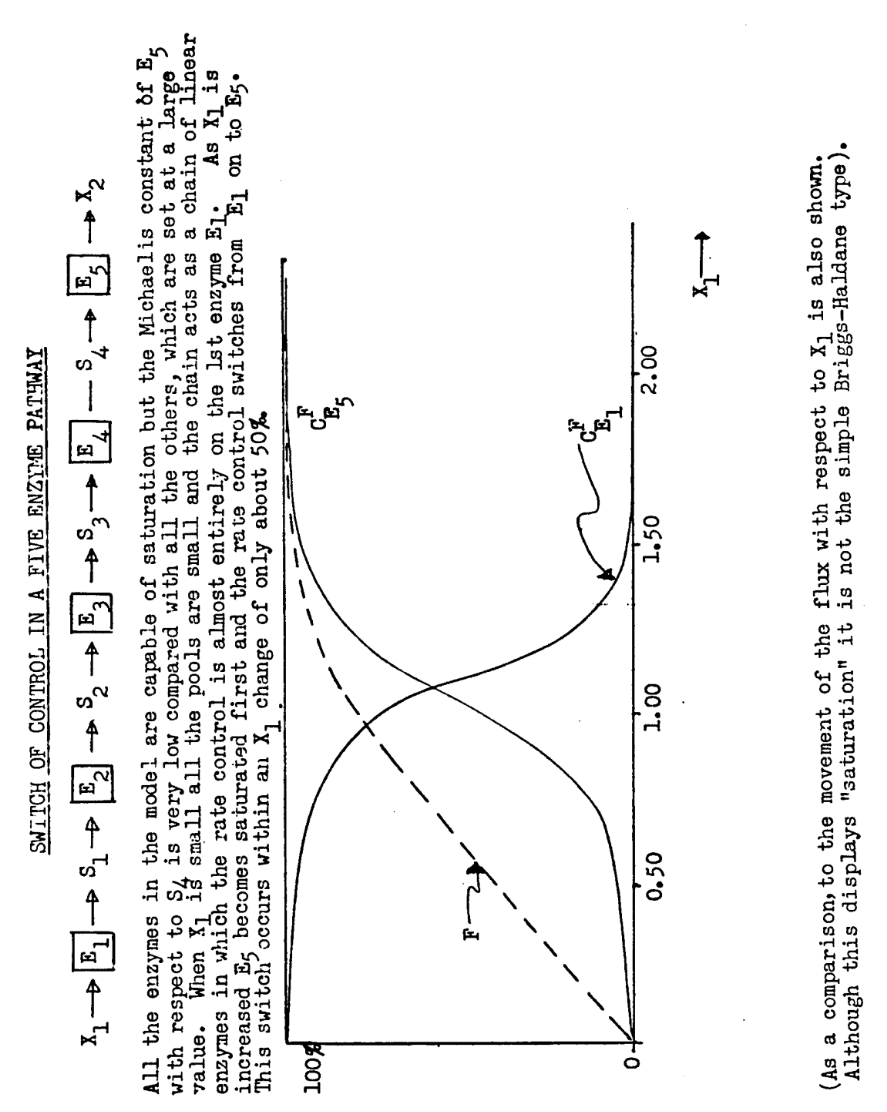
\includegraphics[max width=1\textwidth]{figure5_burnssim.png}
\end{center}

Thus suppose the step corresponding to the locus has two alleles `a' and `b', as shown below.

\begin{center}
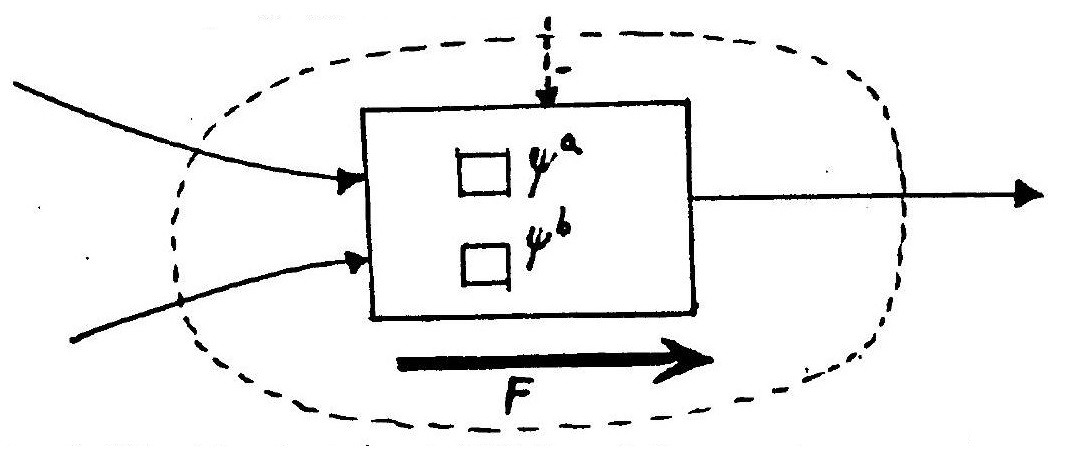
\includegraphics[max width=\textwidth]{2023_01_30_a974a42f7b7381f3f940g-225}
\end{center}

Its `effective' rate expression will be, (p.54)
%
\begin{equation}
F = (1 - \pi)\psi^a + \pi \psi^a
\label{eqn:519}
\end{equation}
%
Where $\psi^{a}$ and $\psi^{b}$ are the complete rate expressions appropriate to the separate alleles in the homozygous state and include enzyme control terms if necessary. Wow when the flux, F, carried by the control terms if necessary. Now when the flux, F, carried by the step alters slightly, due for example to an `a' modulation of the block, the pools $S_{1}, S_{2}, \cdots$, will change only to the extent that $F$ itself has been altered and this will also be true of the known functions of the pools, $\psi^{a}$ and $\psi^{b}$. This is shown in the diagrams below where it should be noted that $\psi^{a} \bumpeq \psi^{b}$ around the existing value, $F^{*}$, of the flux $F$.

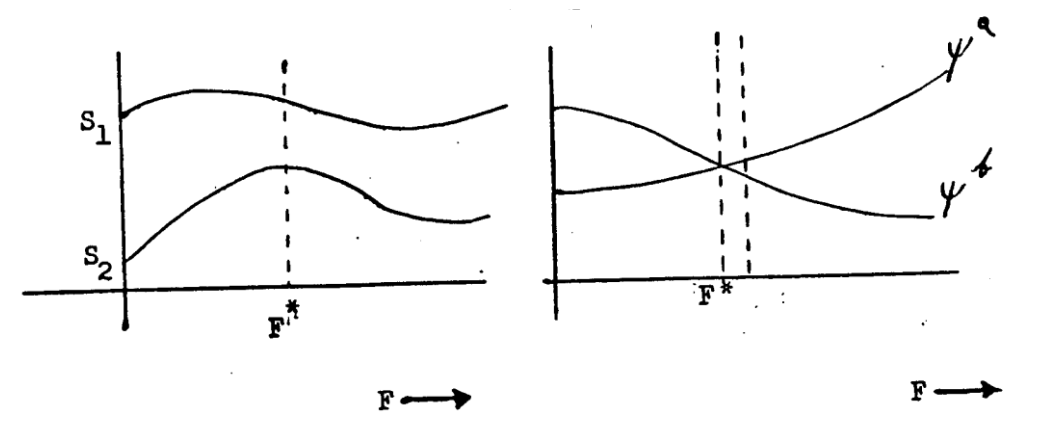
\includegraphics[max width=\textwidth, center]{figure5_flux}

Considering now the composite block, whose rate expression is given by (5.19), in isolation and remembering that the expressions $\psi^{a}$ and $\psi^{b}$ are defined by the flux $F$ we can obtain by differentiation the results that
%
\begin{equation}
C_{1}=1 / 1-\left(\frac{\partial \psi^{a}}{\partial F}\right)_{F=F^{*}}, C_{2}=1 / 1-\left(\frac{\partial \psi^{b}}{\partial F}\right)_{F=F^*} \tag{i}
\label{eqn:520a}
\end{equation}
%
Where $C_{1}$ and $C_{2}$ are the coefficients of the flux $F$ for the block when the locus is homozygous for `a' and `b' respectively.

Next consider the relation $(5.19)$ for $\pi=0,1 / 2,1$, corresponding to the locus being homozygous for `a', heterozygous and homozygous for `b' respectively, and let the respective values of $F$ be $F^{*}, F^{*}+\beta \Delta F^{*}$ and $F^{*}+\Delta F^{*}$.

Remembering that the $\psi$ functions are defined by the flux $F$ this gives rise to the three relations
%
\begin{equation}
F^{*}=\psi^{a}\left(F^{*}\right)  \tag{ii}
\label{eqn:520b}
\end{equation}
%
\begin{equation}
F^{*}+\beta F^{*} = 1/2\left(\psi^{a}\left(F^{*}+\beta \Delta F^{*}\right)+\psi^{b}\left(F^{*}+\beta \Delta F^{*}\right)\right. \tag{iii}
\label{eqn:520c}
\end{equation}
%
\begin{equation}
F^{*}+\Delta F^{*} = \psi^{b}\left(F^{*}+\Delta F^{*}\right) \tag{iv}
\label{eqn:520d}
\end{equation}
%
If $\beta$ can be found from these relations it will be possible to find the dominance since the definition given earlier, in relation $(5.7)$, is equivalent to
%
\begin{equation}
\text { DOM }=2 \beta-1  \tag{v}
\label{eqn:520e}
\end{equation}
%
Where DOM measures the dominance of the allele `b' over the allele `a'. Expanding the $\psi^{a}$ term in (iii) about $F^{*}$, the $\psi^{\text {b}}$ term about $F^{*}+\Delta F^{*}$ and using (ii) and (iv) to provide the 1st parts of these expressions we get
%
$$\beta \cdot \Delta F^{*}=1 / 2\left(\frac{\partial \psi^a}{\partial F} \cdot \beta \cdot F^{*}+\frac{\partial \psi^{b}}{\partial F} \cdot(\beta-1) \cdot \Delta F^{*}\right)$$
%
Which when solved for $\beta$ gives
%
\begin{equation}
\beta=\frac{\frac{\partial \psi^{b}}{\partial F}-1}{\frac{d \psi^{a}}{\partial F}+\frac{d \psi^{b}}{\partial F}-2} \tag{vi}
\label{eqn:520f}
\end{equation}
%
Replacing the derivatives in (vi) by the coefficients $C_{1}$ and $C_{2}$ of relation (i) and using the resulting expression in the relation (v) for DOM we can show that
%
\begin{equation}
\text { DOM }=\frac{C_{1} - C_{2}}{C_{1} + C_{2}}
\label{eqn:521}
\end{equation}
%
The result (5.20), apart from being useful as a numerical estimate in simulation studies, has interesting consequences. Thus in most metabolic situations the coefficients $C_{1}$ and $C_{2}$ can be expected to be +ve for their own flux so that
%
$$
-1 < \mathrm{DOM} < 1
$$
%
This implies that `overdominance' cannot occur between alleles `a' and `b' having only a small effect on pools.

Again the expression (5.20) can be written as $\frac{C_1 / C_2-1}{C_1 / C_2+1}$ and it is clear that even if $C_1$ and $C_2$ are themselves small their ratio can in principle take any positive value. Thus almost complete dominance is quite possible and it will be towards the allele possessing the smaller coefficient. This dominance can occur despite vanishingly small pool and flux responses to the substitution.

\section{Epilogue}

At the outset we stated that our interest was primarily in considering the way in which measures on genetical systems might depend on the underlying genetically specified parameters and on the environment. It is not claimed that we have done more than open up methods for such a consideration and define certain concepts more clearly. However it seems clear in retrospect that this may be a very necessary attempt, aiming, as it does, to understand the quantitative implications of the recent advances in understanding organisms as biochemical systems.

Although considerable work had been carried out by the school of Chance on the \underline{dynamics} of biochemical systems, which served as a useful guide, our own genetical interests dictated a rather different approach in which stress was placed on the stationary solution and its response to parametric variation. 

In this connection the `sensitivity coefficient' of a measure with respect to a differential change in a parameter seems a useful way of describing parametric response and the introduction of a block coefficient enables the relative importance of variation in different functional blocks to be considered. In particular this leads to a clear definition of what is meant by `rate control' in a pathway and the summation property of the flux coefficients (p.85, 3.22) indicates what values of coefficient will indicate a `master' reaction in a pathway. The way in which the block coefficients, which describe the systemic response, are related to the elasticities which describe the behaviour of the separate subunits making up the system, is considered in some detail in CH. III and provides some insight into the way in which the structure of the system and the detailed behaviour of its parts will combine to determine system properties. This treatment makes clear how coefficients of interest within part of a larger system can be determined by an in vivo estimation of the relevant elasticities using data obtained from suitable genetically produced mutants. These theoretical/experimental methods for determining coefficients are contrasted with the more laborious `direct' methods which are also available.

The theory relating system coefficients to elasticities also allows the treatment in CH. III of a number of questions. Thus the use of the pool pattern in a chain of enzymes as a diagnostic for control is extended beyond the linear treatment given in CH I and it is shown under what circumstances the saturation effects become important (p.116). Again it becomes possible to consider whether there are any necessary limits to coefficient values (p.110) and whether the effects of a modulation tend to become attenuated with metabolic distance from the site of the modulation (p.124). Finally it is shown that systems having optima allocation for growth will have. their enzymes distributed in relation to their sensitivity coefficients (p.14l). To some extent all of these theoretical results must remain equivocal in the sense that they are based on particular theoretical assumptions. Accordingly in CH IV emphasis is placed on the idea that computer systems should become available to biochemists and other experimentalists which

Finally in CH.V the implications of our approach for the population genetics of quantitative characters is considered. Of considerable interest here is the theoretical result, specifically demonstrated for a chain of linear enzymes, that considerable dominance and epistasis will arise quite naturally and will persist even when the individual allelic substitutions have a vanishingly small effect. A qualitative argument is provided to show that such a genotype/phenotype relation could, when combined with suitable linkage between the loci, give rise to very different behaviour under selection from that which would be expected on additive assumptions. For more complex systems it is shown that the sensitivity coefficient aids in the estimation of major and minor loci and also can be related, under certain circumstances, to the degree of dominance between two alleles. Once again, however, theory requires to be supported by flexible means for conducting numerical studies on populations of `theoretical organisms'. 

If any claim to a further understanding of the organisation of living things could be made, it would perhaps stress less the particular results shown in this thesis, but emphasise the approach.


